\documentclass[11pt,a4paper]{article}


\usepackage{fancyhdr}
\usepackage{graphicx}
\usepackage{verbatim}
\usepackage{lastpage}
%\usepackage{fullpage}
\usepackage{fancybox}
\usepackage[small,bf]{caption}
\usepackage[usenames,dvipsnames]{color}
\usepackage{hyperref}

% \hypersetup{
%     colorlinks,
%     citecolor=black,
%     filecolor=black,
%     linkcolor=black,
%     urlcolor=black,
% }

\hypersetup{linktocpage}        


\newenvironment{FramedVerb}%
{\VerbatimEnvironment
\begin{Sbox}\begin{minipage}{\textwidth}\begin{Verbatim}}%
{\end{Verbatim}\end{minipage}\end{Sbox}
\setlength{\fboxsep}{8pt}\fbox{\TheSbox}}

\title{Chromatoplots Manual}

\author{StatGraph}
\date{\today}

\setlength{\parindent}{0in}
\setlength{\parskip}{0.5\baselineskip}

\topmargin=-0.45in
\evensidemargin=0in
\oddsidemargin=0in
\textwidth=6.5in
\textheight=9.01in
\headsep=0.25in

\pagestyle{fancy}
\lhead{Manual}
\rhead{Chromatoplots}
% \cfoot{\thepage\, of \pageref{LastPage}}
\cfoot{\thepage}
\renewcommand\headheight{24pt}
% \renewcommand\footrulewidth{0.4pt}

\usepackage{Sweave}
\begin{document}
\maketitle\newpage
\tableofcontents\newpage
% \listoftables\newpage
% \listoffigures\newpage

\section{Introduction}
Metabolomics experiments often rely on Gas Chromatography - Mass
Spectrometry (GC-MS) instruments for measuring the levels of
metabolites. We have developed numerical methods and graphical
diagnostics for converting raw GC-MS data into a dataset specifying
the amount of each metabolite in each sample. In this manual, we
present basic workflow and diagnosic windows.

This manual doesn't include the GUI yet, will be added later. And this
manual doesn't focus on the algrithm, algrithm will be elucidated in
another document later.

Now it's just for developer's communication, will be fullfilled while
developing this package.

\section{Installation}

Please use the latest version of the following package, you can check
out ``commandr'' and ``chromatoplots'' from their svn, and ``xcms''
,''irange'', from Bioconductor\footnote[1]{www.bioconductor.org} dev 2.6 pool.

\textbf{chromatoplots}\\
svn://had.co.nz/statgraphics/chromatoplots/trunk/chromatoplots

\textbf{commandr}\\
svn://had.co.nz/statgraphics/commandr/trunk/commandr

\textbf{xcms}\\
http://www.bioconductor.org/packages/2.6/bioc/html/xcms.html

\textbf{IRanges}\\
http://www.bioconductor.org/packages/2.6/bioc/html/IRanges.html

Check the system and package dependencies before you install chromatoplots,
install xcms first, then commandr, install chromatoplots last.
\newpage

\section{Workflow}
\subsection{Arrange Your File}
First of all, you need to arrange all your raw data based on your
experimental design.

\begin{figure*}[h!t!b!p]
\begin{center}
  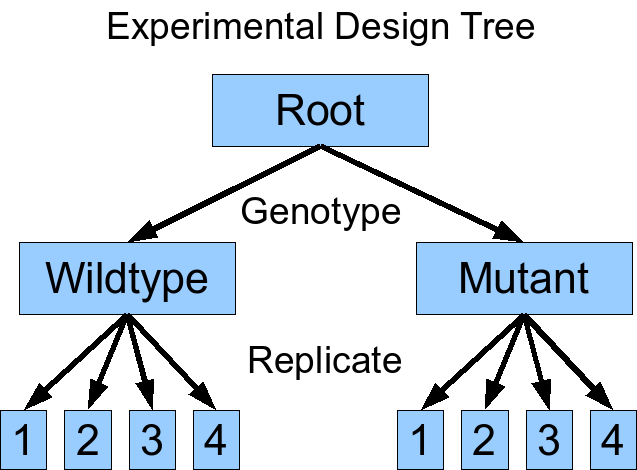
\includegraphics[width=2in]{exp-design-tree.png}
\caption{\label{fig:genprofile}Experimental design}
\end{center}
\end{figure*}
In this study, my experimental design looks like this.
\begin{figure*}[h!t!b!p]
\begin{center}
  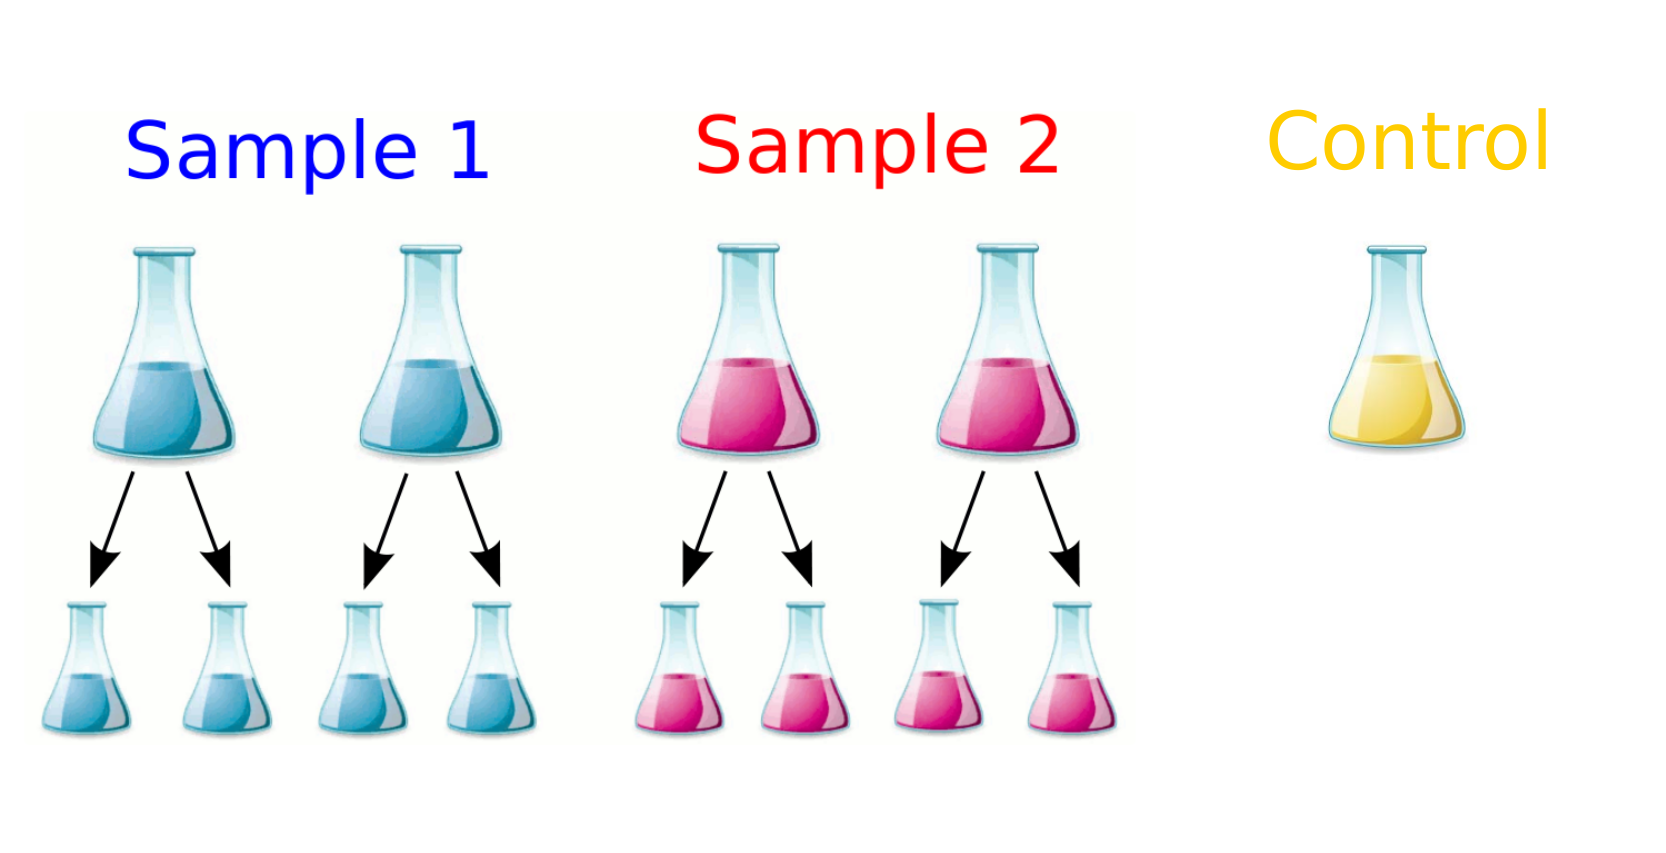
\includegraphics[width=3in]{design.png}
\caption{\label{fig:genprofile}My calibrated data has two treatment, each treatment has four replicates.}
\end{center}
\end{figure*}

So I arranged my file in the following way.
\begin{verbatim}
./raw/s1:
M0101A.CDF  M0101B.CDF  M0102A.CDF  M0102B.CDF

./raw/s2:
M0201A.CDF  M0201B.CDF  M0202A.CDF  M0202B.CDF
\end{verbatim}
\newpage

\subsection{Raw Data Input}
\subsubsection*{Command Line}
Specify a CDF data which contains GC-MS processed raw data by using
the following command, and generate \emph{profile
  matrix}\footnote[1]{Profile matrix has a row for each mass and a
  column for each scan, in order of time.}.

\begin{verbatim}
> file <- "raw/s1/M0101A.CDF"
> raw <- loadSample(file)
> raw_prof <- genProfile(raw) # generate profile matrix
\end{verbatim}
\subsubsection*{Graphic Diagnose}
To call a diagnostic windows for this stage.
\begin{verbatim}
> explore(raw_prof)
\end{verbatim}
\begin{figure*}[h!t!b!p]
\begin{center}
  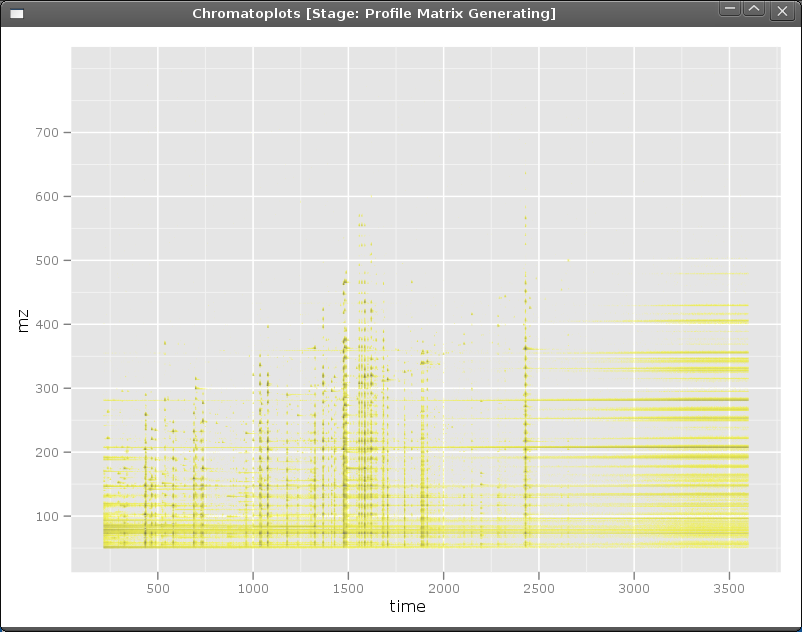
\includegraphics[width=4in]{genprofile.png}
\caption{\label{fig:genprofile}Image of log of the profile
  matrix. Horizontal axis is time, and vertical axis is m/z. The color
  scale ranges from yellow to black. The darker the color, the higher
  the intensity. Gray indicates a time and m/z combination where
  nothing is detected.}
\end{center}
\end{figure*}
\subsubsection*{Low Level Graphic Functions}
\begin{verbatim}
image(object) #profile matrix, slow(more than one minute)
\end{verbatim}

\subsection{Baseline Subtraction}
\subsubsection*{Command Line}
\begin{verbatim}
> cor_prof <- removeBaseline(raw_prof, "median", scanrad = 100)
#if it works great, then accept correction.
> raw <- cor_prof
\end{verbatim}
\subsubsection*{Graphic Diagnose}
\begin{verbatim}
> explore(cor_prof, raw = raw_prof, mz=51)
\end{verbatim}
\begin{figure*}[h!t!b!p]
\begin{center}
  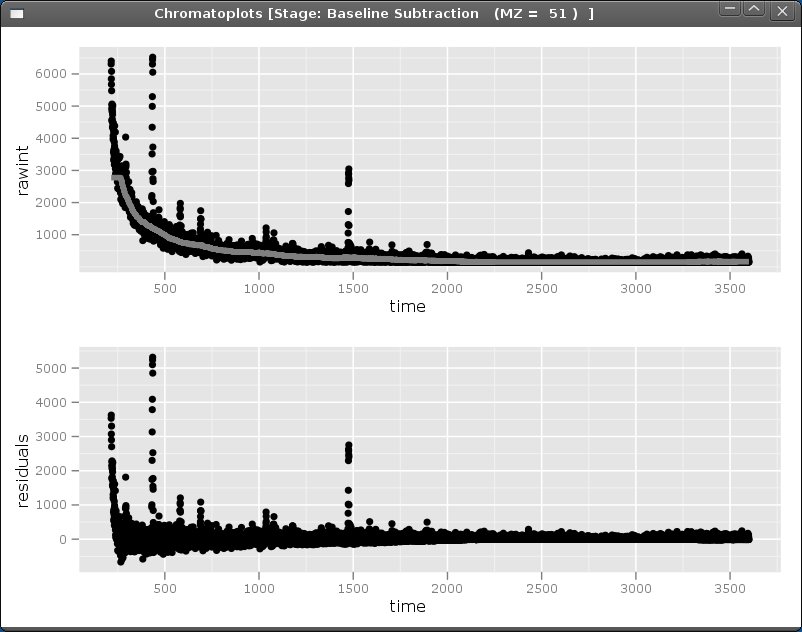
\includegraphics[width=4in]{baseline51.png}
\caption{\label{fig:baseline51}Chromatogram of raw relative
  intensities from the row of the profile matrix corresponding to 51
  m/z. A non-linear baseline is evident.}
\end{center}
\end{figure*}
\subsubsection*{Low Level Graphic Functions}
\begin{verbatim}
explore_prof_filter(object,protocol,raw,mz,subtract=TRUE)
\end{verbatim}


\subsection{Peak Detection}
\subsubsection*{Command Line}
\begin{verbatim}
> peaks <- findPeaks(raw, "gauss") # "gauss" protocol 
\end{verbatim}
You can read another file and do the previous step by simply running 
permorn() command.\\
\begin{verbatim}
> rep_file <- "raw/s1/M0102A.CDF"
> rep_raw <- perform(pipeline(raw), rep_file)
> rep_peaks <- perform(findPeaksProto(peaks), rep_raw)
\end{verbatim}
Or load all replicates within one treatment at once, the first argument specify the directory contains replicates raw files.\\
\begin{verbatim}
> s1_exp <- loadExperiment("raw/s1/", pipeline = pipeline(peaks))
\end{verbatim}

\subsubsection*{Graphic Diagnose}
\begin{verbatim}
> explore(peaks, raw = raw, sample=NA,residuals=TRUE,island=TRUE)
\end{verbatim}

``sample'' controls which sample you want to show; residuals=TRUE if you
want the residual graph, island=TRUE if you want the plot which shows a cutoff line(red)
and peaks(blue) they find for a specific MZ value (identified by user).
\begin{figure*}[h!t!b!p]
\begin{center}
  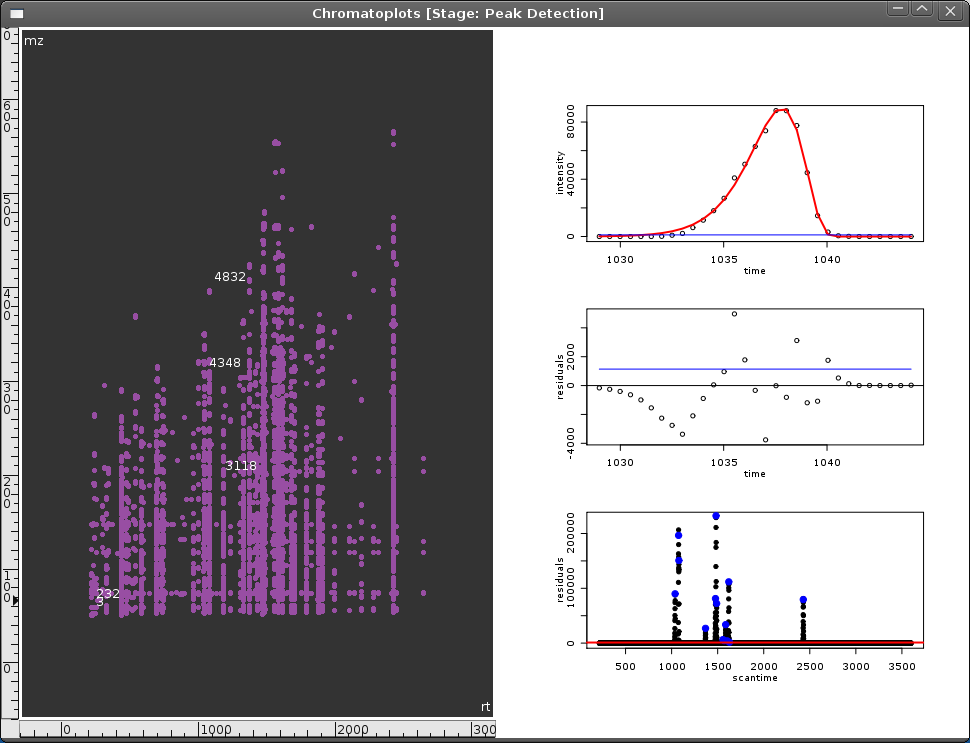
\includegraphics[width=4in]{findpeaks.png}
  \caption{\label{fig:findpeaks}Chromatoplots visualization window for
    the peak detection stage. The user selects points in the left image
    to view the baseline-corrected chromatogram at the corresponding
    m/z. The chromatogram is annotated with the quantile cutoff and
    the maxima of detected peaks(right bottom). On the right top is a GGobi visu-
    alization for exploring the peak fits.}
\end{center}
\end{figure*}
\subsubsection*{Low Level Graphic Functions}
\begin{verbatim}
plot_peak(object,id, raw, cutoff, sample=NA,residuals = FALSE,island=FALSE)
cplotPeaks(obj,raw,mz) #show island only, ggplot2 function
cplotPeaks2(obj,raw,mz) #show island only, basic R graphic,faster

\end{verbatim}


\subsection{Components Detection}
\subsubsection*{Command Line}
To detect components, run the following command, the second method is
essentially the same with the first one, but you can specify a
quantity(TIC) filter and a peaks number filter. The reason here is to
reduce components that contains very few peaks or quantity(if you
want), these components may be falsely assigned to the wrong group,
e.g. those only contains one m/z value maybe identified as one group
with each other.
\begin{verbatim}
> xset_comps <- findComps(s1_exp, "sigma")
> xset_comps_filt <- findComps(s1_exp,"sigma_filt",
                  tic.cutoff=0.69,npeaks.cutoff=0.7)
\end{verbatim}
Then you could load all replicates in the whole expeimental tree at once.
\begin{verbatim}
> samples <- c("raw/s1", "raw/s2")
> s1_s2_xset <- perform(pipeline(xset_comps), samples)
\end{verbatim}

\subsubsection*{Graphic Diagnose}
For graphic diagnose, run the following command, you could compare the
result with filter.
\begin{verbatim}
> explore(xset_comps,sample=1,residual=TRUE,island=TRUE)
> explore(xset_comps_filt,sample=1,residual=TRUE,island=TRUE)
\end{verbatim}
\begin{figure*}[h!t!b!p]
\begin{center}
  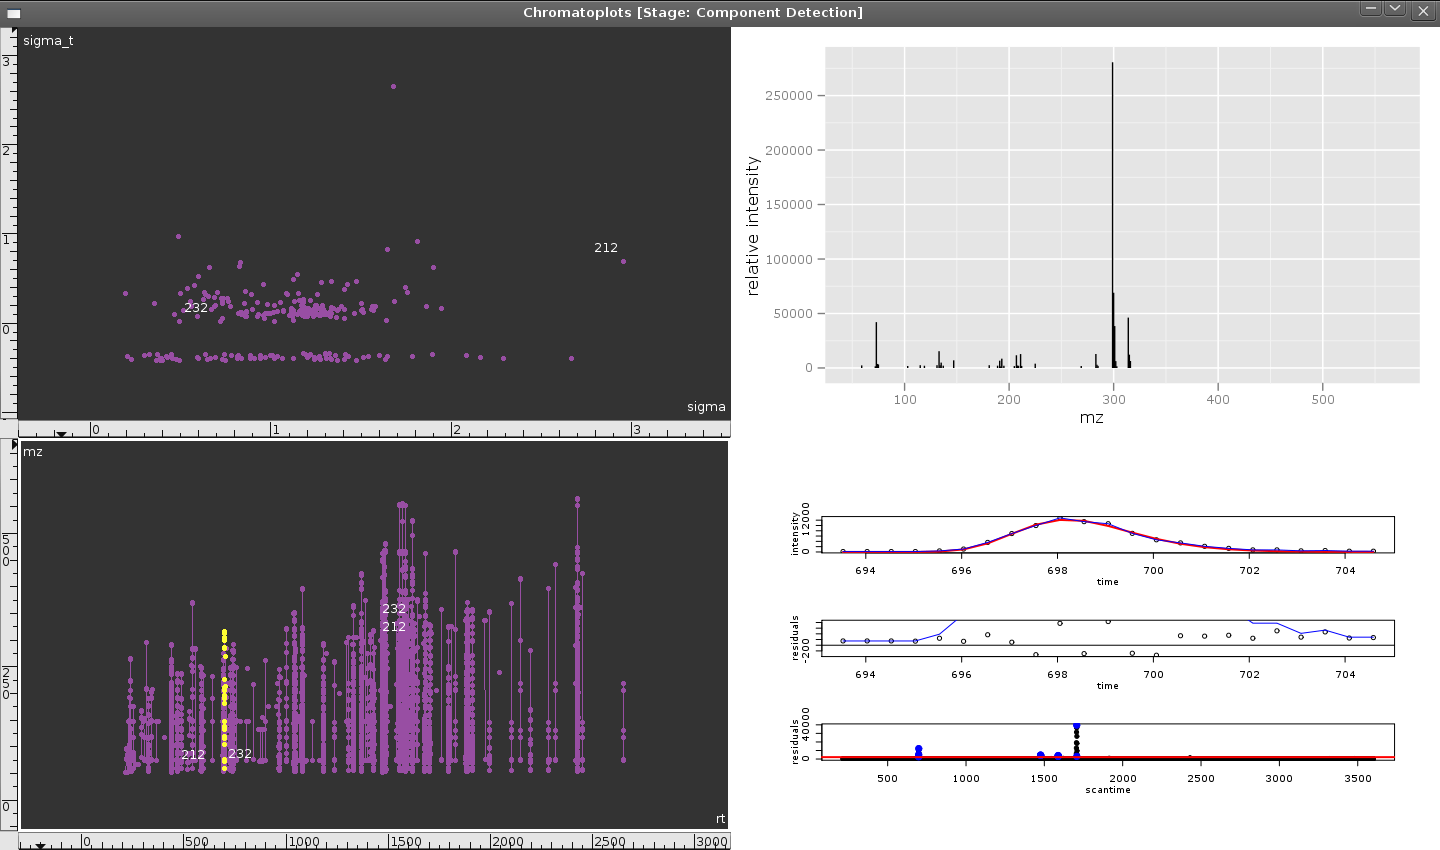
\includegraphics[width=4in]{findcomps1.png}
  \caption{\label{fig:findcomps1}Chromatoplots visualization window
    for the component detection stage. When the user selects
    components in the top scatterplot, the mass spectrum for the
    component is displayed to the right and the corresponding chain of
    peaks is highlighted in the scatterplot on the bottom
    left. Selecting a peak in that plot displays the peak fit to the
    right.}
\end{center}
\end{figure*}
\begin{figure*}[h!t!b!p]
\begin{center}
  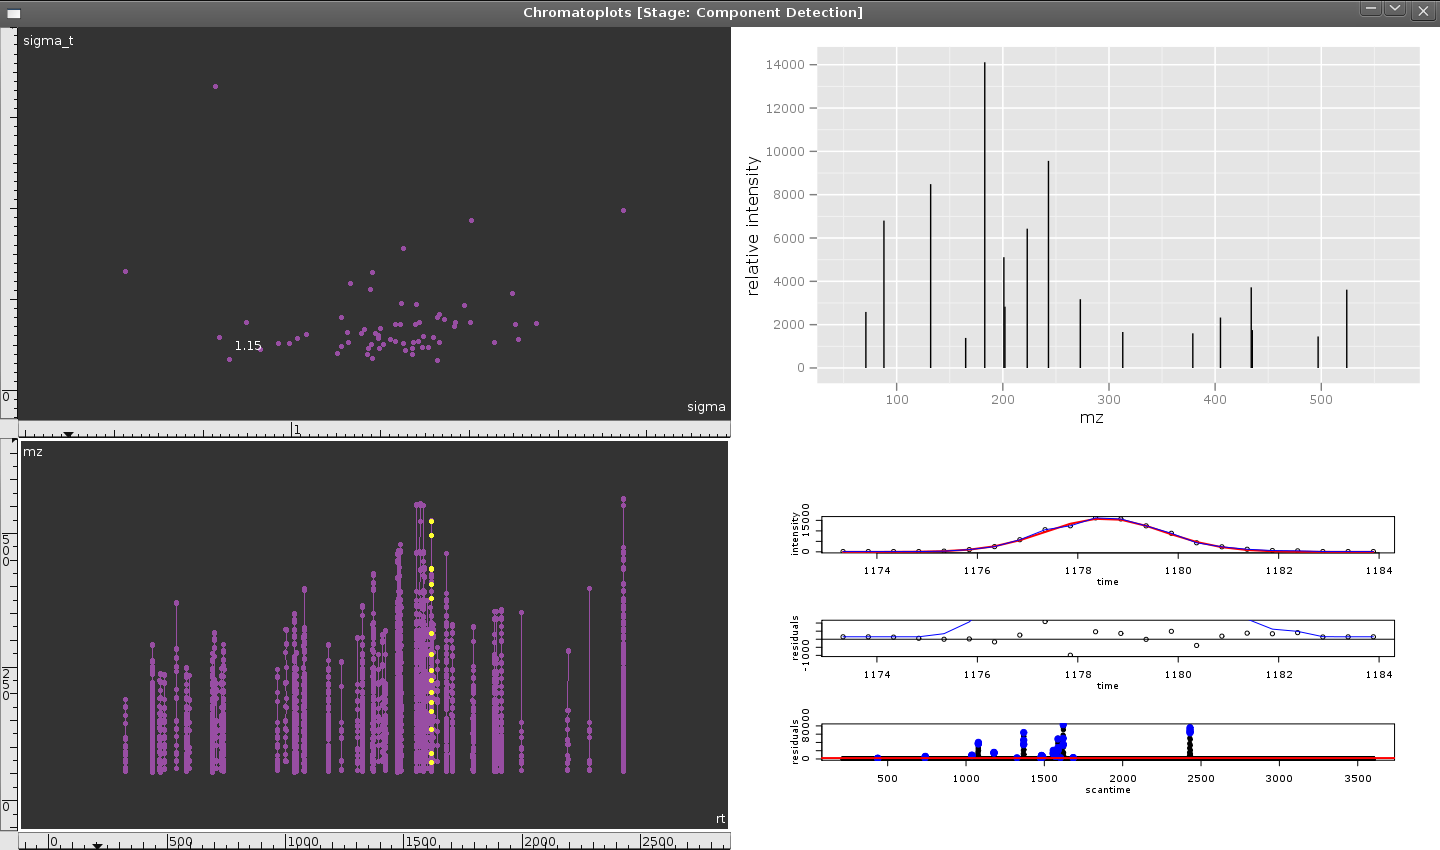
\includegraphics[width=4in]{findcomps2.png}
  \caption{\label{fig:findcomps2}This plot is the same with \label{fig:findcomps1},
but this is after compsfilter, components numbers are reduced a lot.}
\end{center}
\end{figure*}
\subsubsection*{Low Level Graphic Functions}
\begin{verbatim}
plot_comp(peaks, mz_range)
\end{verbatim}

\newpage
\subsection{Grouping Components}
\subsubsection*{Command Line}
Two arguments used here,default dist.cutoff=0.05, rt\_window=-1 which
means default setup never use rt windows filter.
\begin{verbatim}
> xset_groups <- groupComps(s1_s2_xset, "angle")
> xset_groups <- groupComps(s1_s2_xset, "angle",dist.cutoff=0.05,rt_window=1)
\end{verbatim}

\subsubsection*{Graphic Diagnose}
With this interactive graphic, you could diagnose spectra for each
components within one group.
\begin{verbatim}
> explore(xset_groups)
\end{verbatim}
\begin{figure*}[h!t!b!p]
\begin{center}
  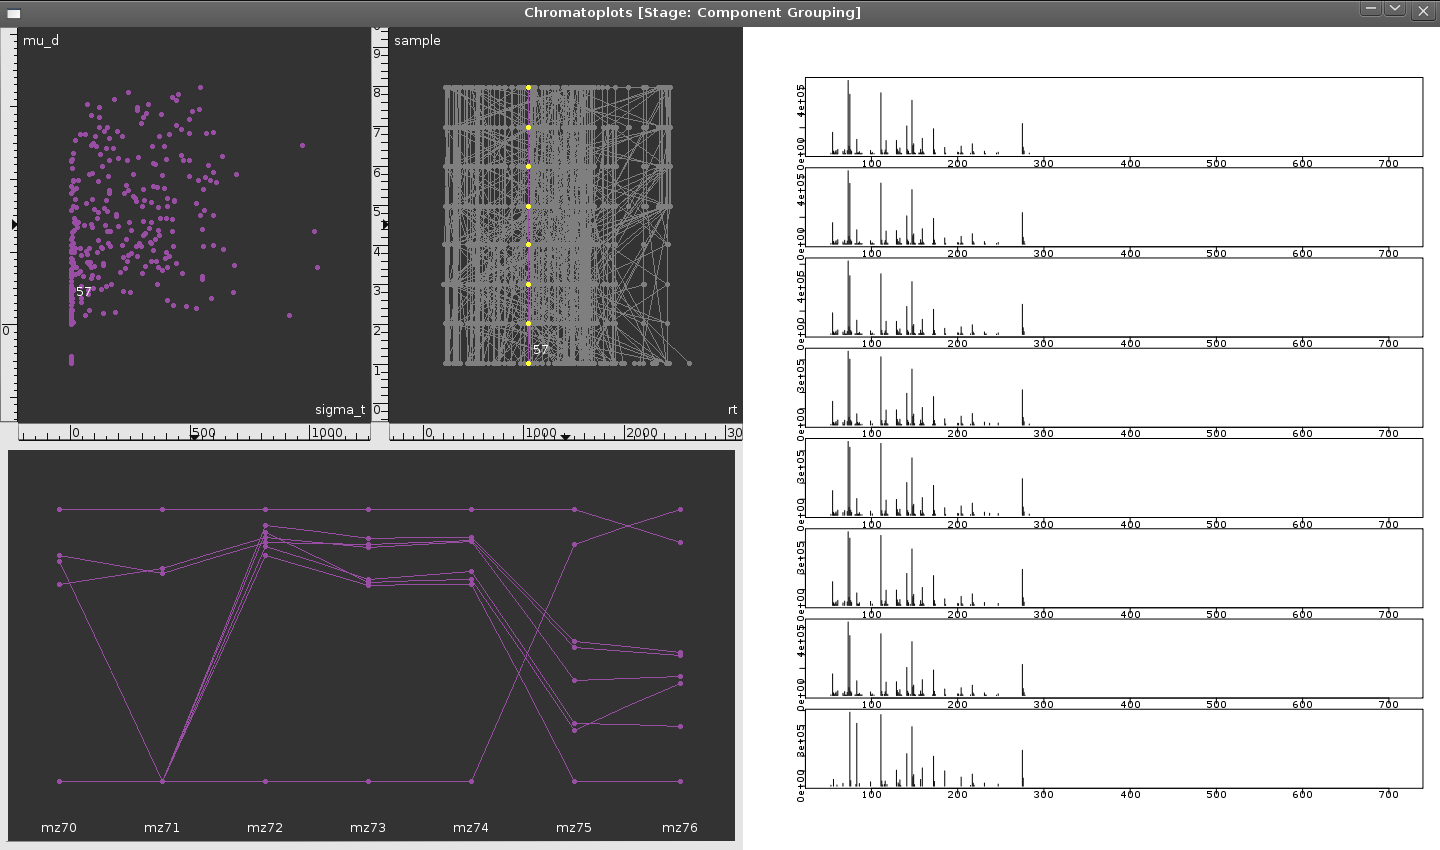
\includegraphics[width=4in]{groupcomps.png}
  \caption{\label{fig:findpeaks}Chromatoplots visualization window for
    the component grouping stage. The user selects a group in the top
    scatterplot to highlight the corresponding chain of components in
    the plot to its right and display the spectra of the components in
    the parallel coordinates plot at the bottom, and plot spectra for
    each components inside that group in the right graphic. }
\end{center}
\end{figure*}
\subsubsection*{Low Level Graphic Functions}
\begin{verbatim}
cplotSpec(object,sample=NA,comp=NA,group=NA,...)
\end{verbatim}

\newpage
\subsection{Retention Time Correction}
\subsubsection*{Command Line}
This stage based on the grouping result, which means if components are
grouped in the wrong way, retention time will not be corrected in the
right way, so you should pay attention to the last stage.
\begin{verbatim}
> xset_rtcor <- rtcor(xset_groups, "rloess")
\end{verbatim}
\subsubsection*{Graphic Diagnose}
We offer two ways to view the retention time, one is heatmap, the other one is
lines, you can specify x-scale, samples you want to diagnose.(not interactive yet)
\begin{verbatim}
> explore(xset_rtcor_filt,raw=xset_groups_filt,geom="heatmap")
\end{verbatim}
\begin{figure*}[h!t!b!p]
\begin{center}
  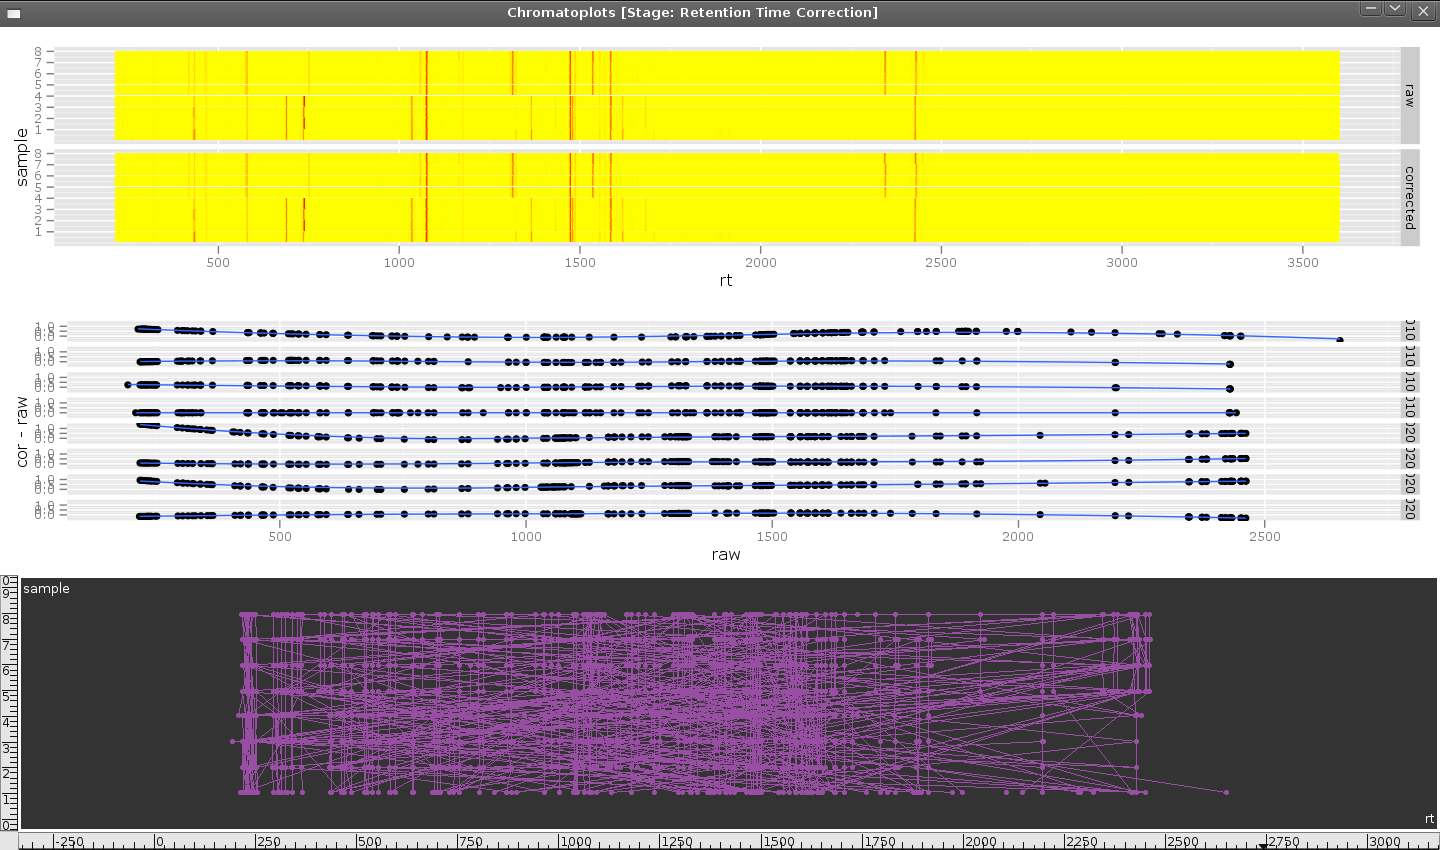
\includegraphics[width=4in]{rt_heat.png}
  \caption{\label{fig:findpeaks}Chromatoplots visualization window for
    the retention time correction stage. Using ``heatmap'' method to
    plot for all the data}
\end{center}
\end{figure*}
\begin{verbatim}
> explore(xset_rtcor,raw=xset_groups,sample=1:2,xscale=c(1000,1500))
\end{verbatim}
\begin{figure*}[h!t!b!p]
\begin{center}
  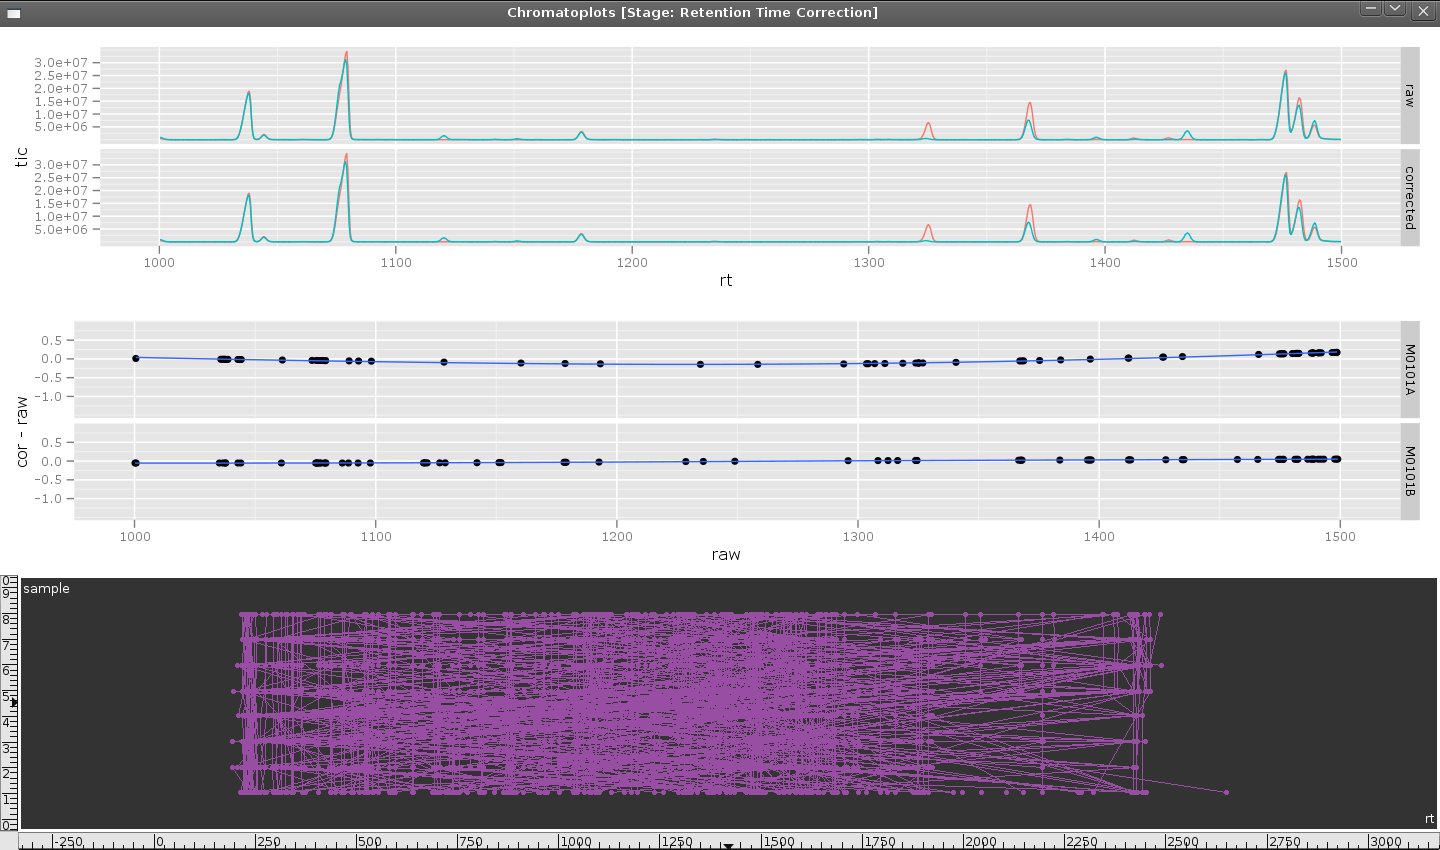
\includegraphics[width=4in]{rt_tic.png}
  \caption{\label{fig:findpeaks}Chromatoplots visualization window for
    the peak detection stage. Using lines to show small group or scale of data}
\end{center}
\end{figure*}
\subsubsection*{Low Level Graphic Functions}
\begin{verbatim}
cplotRT(object,xscale=NA,geom=NA,sample=NA,log=F)#geom=NA or "heatmap"
cplotRtFit(object,raw,xscale=NA,sample=NA) #cor-fit plot
\end{verbatim}


\newpage
\subsection{Summarization}
\subsubsection*{Command Line}
\begin{verbatim}
> xset_sum <- summarize(xset_groups,"common")
\end{verbatim}

\subsubsection*{Graphic Diagnose}
\begin{verbatim}
> explore(xset_sum)
\end{verbatim}
\begin{figure*}[h!t!b!p]
\begin{center}
  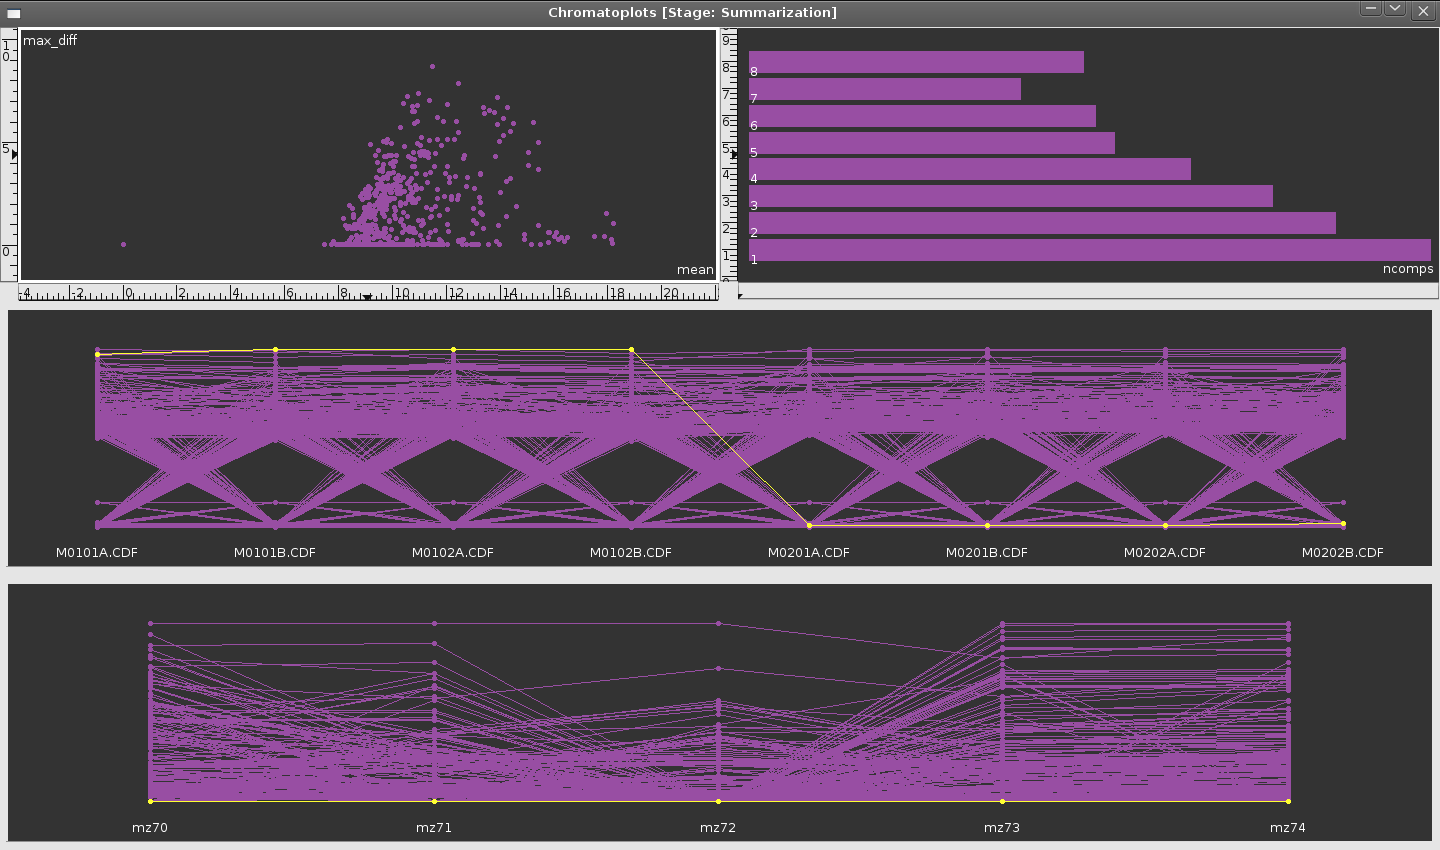
\includegraphics[width=4in]{sum.png}
  \caption{\label{fig:findpeaks}Chromatoplots visualization window for
  the summarization stage. By selecting a group in the top-left
  scatterplot, the user can examine the trend of the group over the
  samples and compare the mass spectra of its components.}
\end{center}
\end{figure*}

\subsection{Normalization}
\subsubsection*{Command Line}
\begin{verbatim}
> xset_norm <- normalize(xset_sum, "scale")
\end{verbatim}

\subsubsection*{Graphic Diagnose}
No diagnose graphic for this stage yet.

\newpage
\subsection{Metabolite Identification}
\subsubsection*{Command Line}
MSP format could be read by AMDIS to identify metabolites based on the
NIST library. So far we only offer MSP transform from our final
result.  Our recommendation is: first read the processed data into
explorase, then find the metabolite of interest in your favorite way,
pick up the id for those metabolite, then use the following command to
finish the transformation. 'id' indicate the metabolite of interest,
and 'file' argument specify a file name you want to output to.
\begin{verbatim}
> dump2msp(xset_norm1_filt,id=c(183,80),file="~/interest.msp")
\end{verbatim}
MSP format looks like this, in each parenthesis, left number indicate M/Z ratio, and 
right number indicate quantity, this list store the information about spectra for 
specific metabolite.
\begin{verbatim}
NAME:ID= 183 
COMMENT:
RI:
CASNO:
RT: 12.31059 
SOURCE:
NUM PEAKS: 116 
( 52      1914)( 53      2737)( 54      1816)( 55     13739)( 56     11831)
( 57     25260)( 58     49057)( 59    340150)( 60     28146)( 61     19998)
( 66      8410)( 67      1950)( 69      3679)( 70     18527)( 71     19182)
( 73   2520939)( 74    216013)( 75    163938)( 76      8531)( 77      2867)
( 82      1302)( 83      3869)( 84      8377)( 85     22143)( 86    738410)
( 87     78753)( 88     31147)( 89      5262)( 95      6570)( 97      1239)
( 98      4172)( 99     16189)(100    451355)(101    100048)(102     46618)
(103     35702)(104      6098)(105     13001)(106      1567)(109      1304)
(112      2416)(113     19520)(114     19720)(115     33595)(116     57323)
(117    159767)(118     26505)(119     52013)(120      6254)(121      2898)
(123      2658)(128      5611)(129     13716)(130    198813)(131    187114)
(132     54134)(133    600902)(134     88626)(135     45430)(136      4035)
(142      4978)(143      5232)(144     59164)(145     15154)(147   1876247)
(148    288850)(149    144728)(150     14222)(151      3035)(156      1950)
(158    100146)(159     28280)(160     37288)(161     12054)(162      3850)
(171      3126)(172     80766)(174   8348546)(175   1543325)(176    663500)
(177    103438)(178     17975)(179      3491)(187      5887)(188     58814)
(189     17957)(190     17487)(191      7612)(192      2102)(202     33007)
(203      6666)(204     41724)(205     11967)(206      5912)(207      1754)
(218      7095)(219      1808)(221      1818)(232      4204)(234      1909)
(246    120672)(248   1948382)(249    492673)(250    244634)(251     42950)
(252      9950)(262     10635)(263      2754)(264      1341)(276    665575)
(277    174492)(278     86643)(279     15637)(280      3916)(291      3736)
(292      1191)

NAME:ID= 80 
COMMENT:
RI:
CASNO:
RT: 17.92231 
SOURCE:
NUM PEAKS: 30 
( 68     14601)( 82      1207)( 84      3577)( 86     90239)( 98      5911)
(100     55826)(112      6396)(114     15901)(126      2180)(140     15216)
(142     43639)(144     24571)(154      1505)(156     21899)(158     14960)
(170      3668)(171      1918)(172     57686)(174   1541131)(175    285225)
(176    121220)(186      4869)(200      3673)(214     13901)(246     79569)
(247     17734)(248      6937)(288      5245)(302      1693)(304    591876)

\end{verbatim}

\newpage
\section{Other Graphic Function}
Keep updating ...
\begin{verbatim}
cplotTIC (object,xintercept=NA,xscale=NA,color=NA) # plot TIC
\end{verbatim}

\newpage
\section{Workflow Fast Reference}
\begin{verbatim}
> file <- "raw/s1/M0101A.CDF"        
> raw <- loadSample(file)     # load raw data
> raw_prof <- genProfile(raw) # generate profile matrix
> explore(raw_prof)           # view profile matrix, slow 
> cor_prof <- removeBaseline(raw_prof, "median", scanrad = 100)
> raw <- cor_prof #if it works great, then accept correction.
> explore(cor_prof, raw = raw_prof, mz=51) 
> peaks <- findPeaks(raw, "gauss") # "gauss" protocol 
> rep_file <- "raw/s1/M0102A.CDF"
> rep_raw <- perform(pipeline(raw), rep_file)
> rep_peaks <- perform(findPeaksProto(peaks), rep_raw)
> s1_exp <- loadExperiment("raw/s1/", pipeline = pipeline(peaks))
> explore(peaks, raw = raw, sample=NA,residuals=TRUE,island=TRUE)
> xset_comps <- findComps(s1_exp, "sigma")
# you can use filter here
> xset_comps_filt <- findComps(s1_exp,"sigma_filt",
                  tic.cutoff=0.69,npeaks.cutoff=0.7)
> samples <- c("raw/s1", "raw/s2")
> s1_s2_xset <- perform(pipeline(xset_comps), samples)
> explore(xset_comps,sample=1,residual=TRUE,island=TRUE)
> xset_groups <- groupComps(s1_s2_xset, "angle")
# or use dist.cutoff and rt_window filter at the same time. 
> xset_groups <- groupComps(s1_s2_xset, "angle",dist.cutoff=0.05,rt_window=1)
> explore(xset_groups)
> xset_rtcor <- rtcor(xset_groups, "rloess")
> explore(xset_rtcor_filt,raw=xset_groups_filt,geom="heatmap")
# or use other ways to view this stage
> explore(xset_rtcor,raw=xset_groups,sample=1:2,xscale=c(1000,1500))
> xset_sum <- summarize(xset_groups,"common") #summarization
> explore(xset_sum)
> xset_norm <- normalize(xset_sum, "scale")  #normalization
> library(explorase)
# use explorase to pick up interest id.
> explorase(as(xset_norm,"ExpressionSet"))
# transfrom this id to MSP format 
> dump2msp(xset_norm1_filt,id=c(183,80),file="~/interest.msp") 
# Identify your metabolite
\end{verbatim}
\newpage
\section{Update List}
\subsection{2009-11-1}

\begin{itemize}
\item {Metabolite identification: dump2msp() transform final data to MSP format}
\item{ Remove legend for profile matrix.}
\item{ Using stack\_plots to show profile matrix.}
\item{ Baseline subtraction: add arguments mz to explore() and related low level function, could be used for 
interactive from raw profile matrix later.}
\item{ Find Peaks: Dignostic windows fixed, add interactive plot for 
mz, and find a way to embed three figures in one box.}
\item{ Find comps: remove 'prof' and 'raw' argument, compute them from the object based on
protocol@alpha, add some other argument.}
\item{ ProcessProtoRaw,desn't work so far, so use sample argument to retrieve the file
path from phenoData slot.}
\item {Retention time add some diagnostic graphic}
\item {Grouping components:Add interactive spectra diagnostic window}
\item {remove undifined protocol from namespace, so the package can be complied}
\item {Add retetion time to feature data}



\end{itemize}
\end{document}
